\section{Cost variables}
Computing costs occur for blockchain applications, and because the blockchain is decentralized, there needs to be a reward system for the people that provide the service of confirming the transactions.
Therefore, a blockchain application can be significantly more expensive than a comparable centralized service. The costs of a single transaction on the Ethereum blockchain is dependant on at least 5 variable factors: 1. The operations being done 2. The gas costs assigned to those operations 3. The desired speed of which transactions are executed 4. The value of ether 5. The compiler being used.

When a node wants to submit a transaction to the blockchain or create a new contract, a certain amount of {'}gas{'} has to be offered to so called {'}block miners{'}. For the purpose of a cost model, gas is as a real money cost and should be treated as a currency.

\textbf{1 The operations being done}: The amount of gas that has to be paid is determined by the assembly code of the transaction. There are currently 31 possible operations, each one has a gas price tag attached to it.

\par
\textbf{2 The gas costs assigned to those operations}: Gavin Wood has created a list of 31 operations and their prices, and these are in use today. For example, a transaction costs 21000 gas and a SHA3 hash operation costs 30 gas. In general, it can be stated that more complicated contracts and transactions cost more gas. Interestingly, the different gas prices for operations are not necessarily proportional of the actual computational work needed, but were set by the Ethereum core team and accepted by the majority Ethereum users. Because of the non-proportionality, some assembly instructions will change their gas prices in the future for rebalancing purposes when the majority of nodes upgrade to the Metropolis hard fork. This hark fork is not yet certain to happen, but will likely do so as this hard fork is pushed by Ethereum inventor Vitalik Buterin. For example, the cost of a CALL operation will be increased from 700 to 4000 gas with the Metropolis upgrade.
In summary, gas prices are determined by the community and are heavily influenced by the Ethereum Foundation. Gas prices can change over time, so that the very same transaction can cost more or less gas depending on the time when it is committed.

\par
\textbf{3 The desired speed of which transactions are executed}: How much a gas costs is dependant on the users of the Ethereum network and unlike the previously mentioned operation price table, the gas-to-ether conversion rate is not hardcoded into the Ethereum, but determined by the users dynamically. The default configuration of go-ethereum\footnote{ https://github.com/ethereum/go-ethereum/blob/fff16169c64a83d57d2eed35b6a2e33248c7d5eb/eth/config.go\#L45}, which is the standard implementation for Ethereum, sets a gas price of 20 shannon\footnote{ Shannon is $10^{-9}$ Ether. A shannon is also known as a 'Gwei'. In the context of gas prices, 'shannon is more commonly used.}, although it is configurable. When the gas price is set to 20 shannon in a miners client, the miner will only mine transactions that offer a gas price of 20 or more. When the gas price is set to 20 shannon in a client that wants to send a transaction, the client will automatically offer that amount. The average gas price chart from etherscan.io shows that the clients of the network in general go with the default configuration value, 1 gas equals to approximately 23 shannon on average.
The reason that the real average gas price is a bit higher than 20 shannon is because clients can voluntarily offer a higher price for a transaction, like for example a gas price of 24 shannon. This has the advantage that the transaction likely will be fulfilled quicker. The mechanics of mining are similar to those of a stock market. Let's say that a stock is worth 100 USD and is being actively traded on an exchange. If a buyer is willing to buy the stock at an overvalued price of for example 102 USD, his offer will jump to the top of the order book and will be filled the quickest. For our application, it could be desirable to pay a premium for faster transaction mining.
The default price of gas is regularly debated in the Ethereum community and was already changed once in March 2016 when the price for Ether soared. The gas price was then reduced from 50 shannon to 20 shannon. Now that the Ether price is in a different magnitude, another correction might be included in the next hard fork. At the time of writing, the gas price equilibrium would be 16 shannon according to the calculation from etherchain.org.
On May 7th 2017, ethgasstation.info announced\footnote{https://medium.com/@ethgasstation/the-safe-low-gas-price-fb44fdc85b91} that 10\% of the network hashpower is accepting a gas price of only 2 shannon. The site is promoting lower gas prices and is encouraging Ethereum users to change the settings to allow lower gas prices. According to the same site, a transaction that offers 2 shannon per gas, the mean transaction confirmation time is 119 seconds. For 20 shannon and 28 shannon, the transaction confirmation time is 44 and 30 seconds respectively.

\begin{figure}[H]
\centering
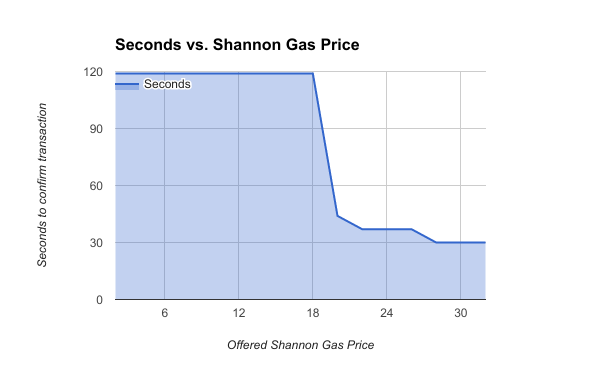
\includegraphics[width=0.85\textwidth]{gas-vs-transaction-time.png}
\caption{Average time until transaction is confirmed. Made with data from ethgasstation.info on May 8th.}
\label{fig:gas}
\end{figure}

In Figure ~\ref{fig:gas}, it can be seen that a node that offers a higher reward for a transaction will get confirmed 4 times faster on average. The user has to decide based on that information, how much he wants to pay.

\textbf{4 Price of Ether}: Ether can either be mined or can be purchased on an exchange. The Ether price on exchanges is highly volatile. On January 1st 2017, the price of an ether was \$8.22. on May 7th 2017, it was \$96.24, according to Coinbase. Ether has also already seen a price drop of over \% when a smart contract called "TheDAO" was hacked.

\textbf{5 The compiler being used}: The final variable is the deviation of gas estimates when using different compilers. This was discovered when receiving different gas estimates for the same contract when upgrading the compiler. To illustration the effect, let's consider the following smart contract:

\definecolor{dkgreen}{rgb}{0,0.6,0}
\definecolor{gray}{rgb}{0.5,0.5,0.5}
\definecolor{mauve}{rgb}{0.58,0,0.82}

\lstset{frame=tb,
  language=Java,
  aboveskip=3mm,
  belowskip=3mm,
  showstringspaces=false,
  columns=flexible,
  basicstyle={\small\ttfamily},
  numbers=none,
  numberstyle=\tiny\color{gray},
  keywordstyle=\color{blue},
  commentstyle=\color{dkgreen},
  stringstyle=\color{mauve},
  breaklines=true,
  breakatwhitespace=true,
  tabsize=3
}

\lstinputlisting{snippets/compiler-deviation.sol}


The gas estimate was 318'552 gas when compiled with Version 0.4.8 of the Solidity Compiler (solc), but slightly different in other compilers:

\begin{center}
  \begin{tabular}{ l | r }
    \hline
    \textbf{Change, \textit{ceteris paribus}} & \textbf{Cost} \\ \hline
    Base case & 318552 gas \\ \hline
    Compiling with solc 0.4.9 instead of solc 0.4.8 & 329054 gas \\ \hline
    Estimate given by Ethereum Wallet 0.8.9 & 318488 gas \\ \hline
    Deployed in Main Network (actual cost) & 318487 gas \\
    \hline
  \end{tabular}
\end{center}

Even when removing just whitespace from the contract, the gas cost can, but does not have to change:

\begin{center}
  \begin{tabular}{ l | r }
    \hline
    \textbf{Change, \textit{ceteris paribus}} & \textbf{Cost} \\ \hline
    Changing the name from "DdosMitigation" to "Ddos" & 318552 gas (no change) \\ \hline
    Removing line 14 (whitespace) & 318488 gas \\ \hline
    Removing line 10 (whitespace) & 318552 gas (no change) \\
    \hline
  \end{tabular}
\end{center}

Given that all the deviations discovered skewed the total gas cost by not more than 4\%, this variable is omitted from our cost model for simplicity.
